\section{The Assistant Grammar}
\label{sec:grammar}
\begin{figure}
	\centering
     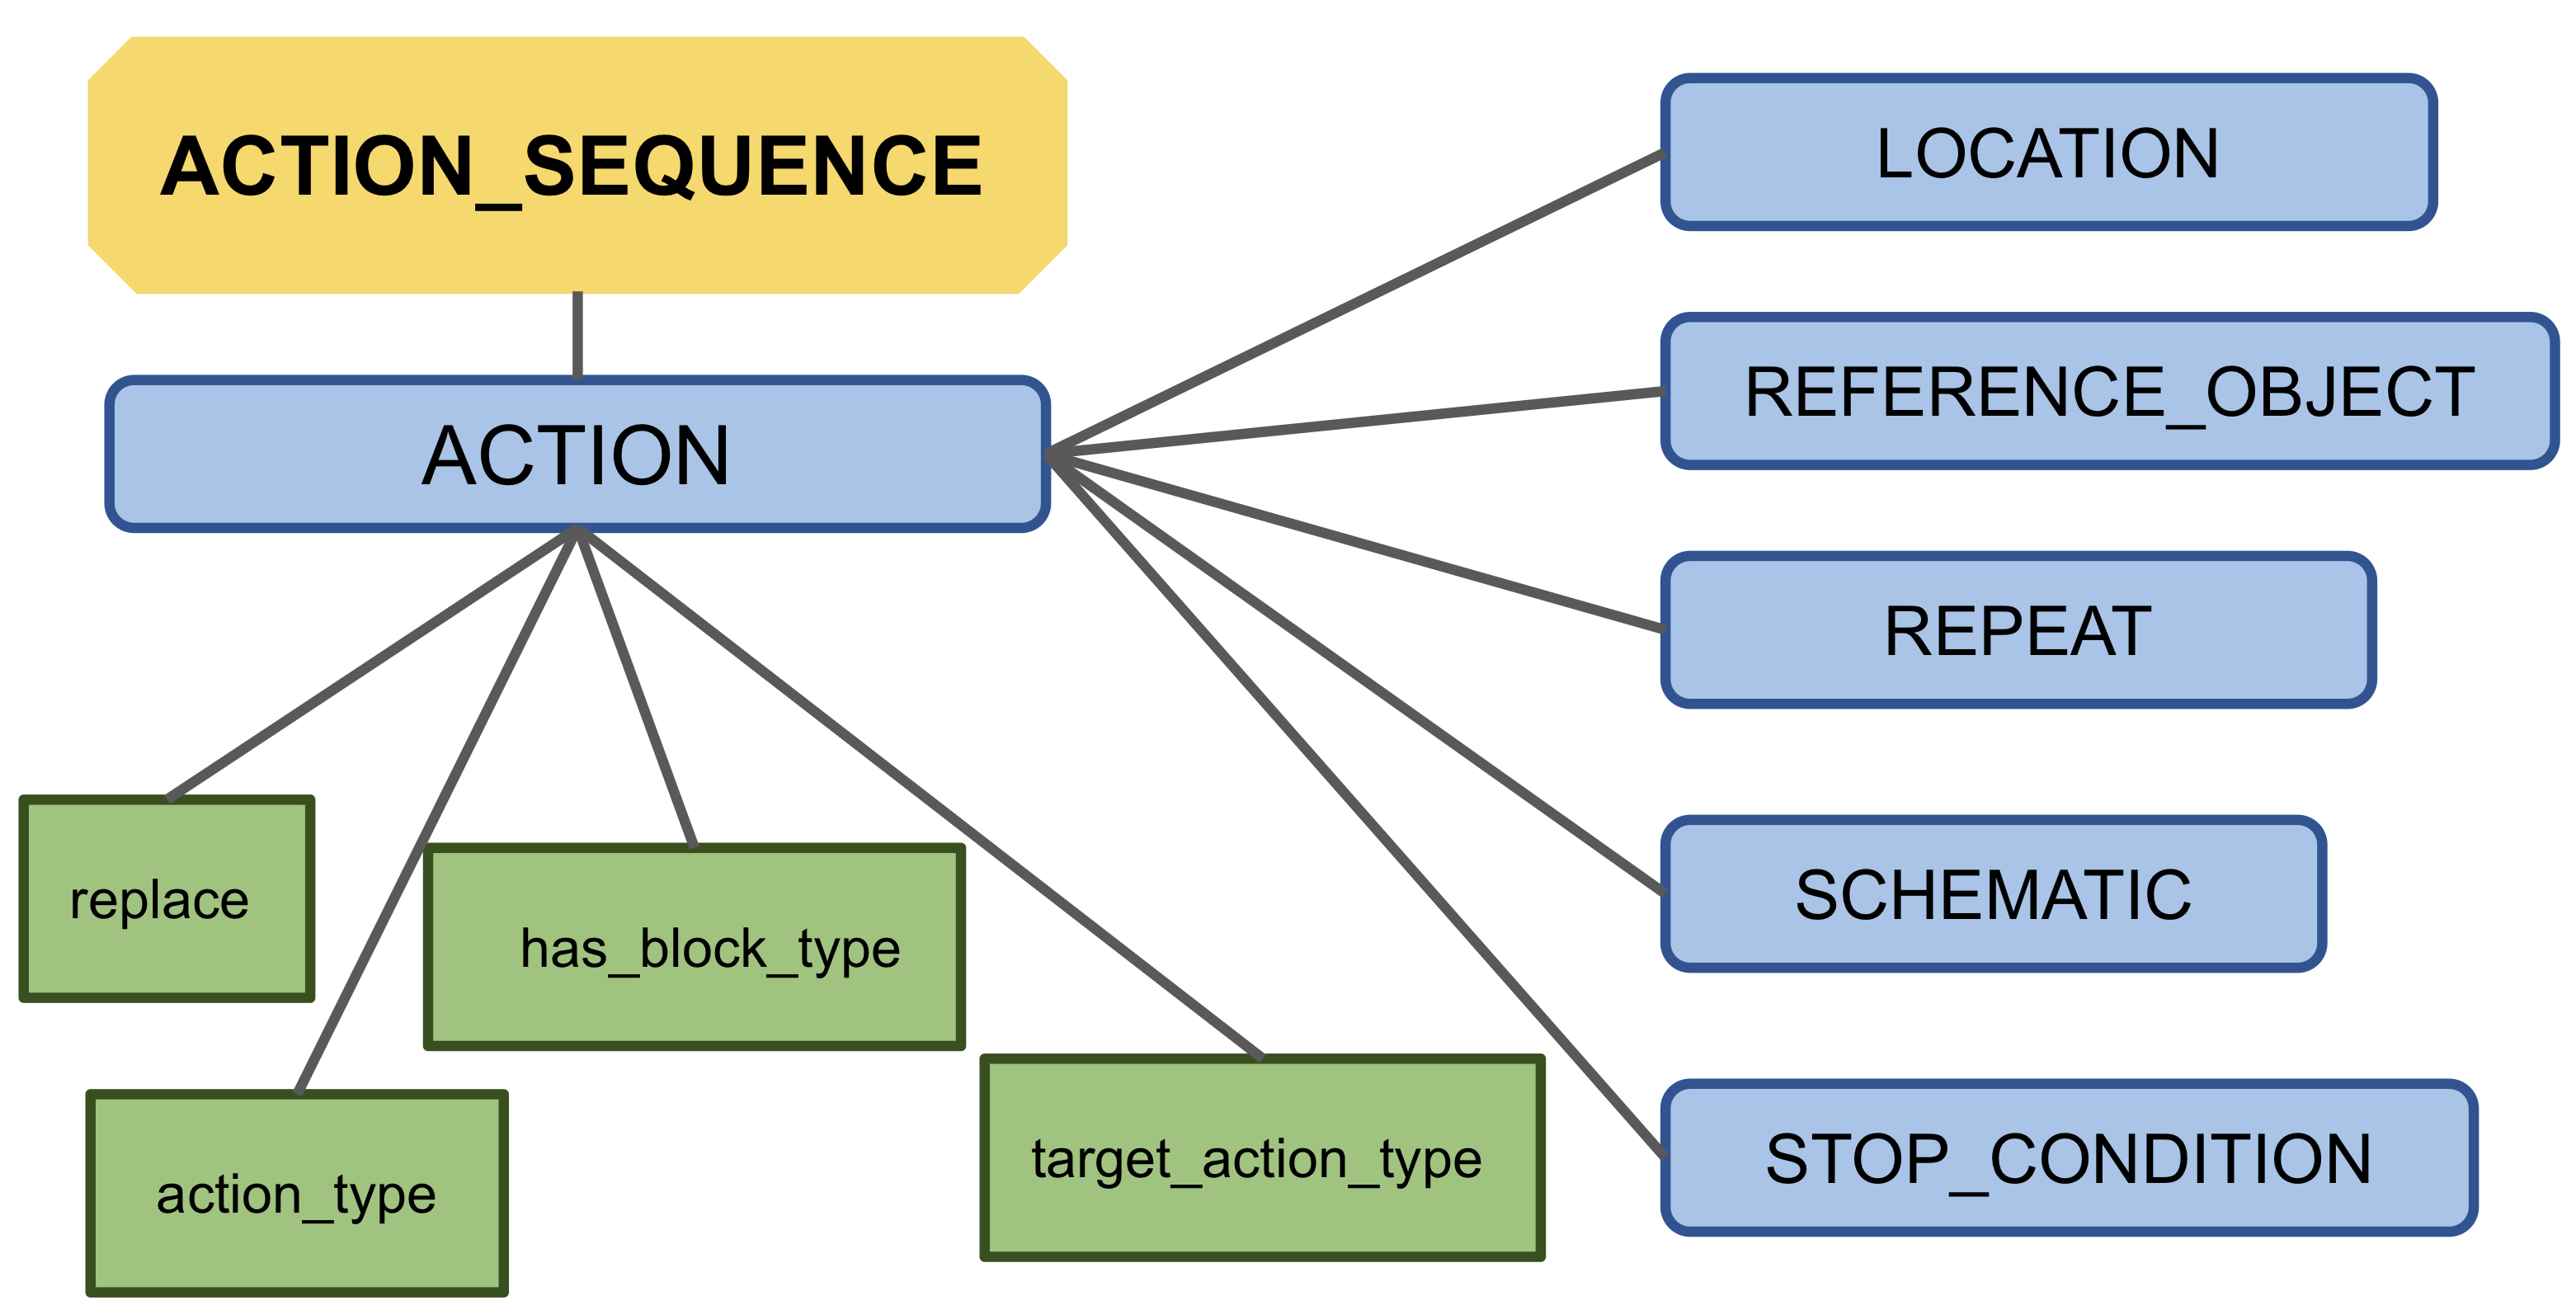
\includegraphics[width=.72\linewidth ]{figures/AS.png}

    \caption{The basic structure of the \textsc{action\_sequence} branch of the assistant's grammar.   The gold octagon is an internal node whose children are ordered,  blue rectangles are regular internal nodes,  and green rectangles are categorical leaf nodes.   Not all combinations of children of \textsc{action} are possible, see the full list of possible productions (and the productions for \textsc{put\_memory} and \textsc{get\_memory})  in the Appendix.}
    \label{fig:AS}
    
\end{figure}


 In this section we summarize a grammar for generating logical forms that can be interpreted into programs for the agent architecture described in \cite{gray2019craftassist}.

\subsection{Agent Action Space}
The assistant's basic functions include moving, and placing and destroying blocks.  Supporting these basic functions are methods for control flow and memory manipulation.  

\smallskip

\noindent{\bf Basic action commands: } The assistant can \textsc{move} to a specified location; or \textsc{dance} with a specified sequence of steps.  It can \textsc{build} an object from a known schematic (or by making a copy of a block-object in the world) at a given location, or \textsc{destroy} an existing object.  It can \textsc{dig} a hole of a given shape at a specified location, or \textsc{fill} one up. The agent can also be asked to complete a partially built structure however it sees fit by \textsc{freebuild}.  Finally, it can \textsc{spawn} a mob (an animate NPC in Minecraft).    

\smallskip

\noindent{\bf Control commands: } Additionally, the agent can \textsc{stop} or \textsc{resume} an action, or \textsc{undo} the result of a recent command.   Furthermore, the assistant can \textsc{loop} given a task and a stop-condition. Finally, it needs to be able to understand when a sentence does not correspond to any of the above mentioned actions, and map it to a \textsc{noop}.

\begin{figure}
    \centering
    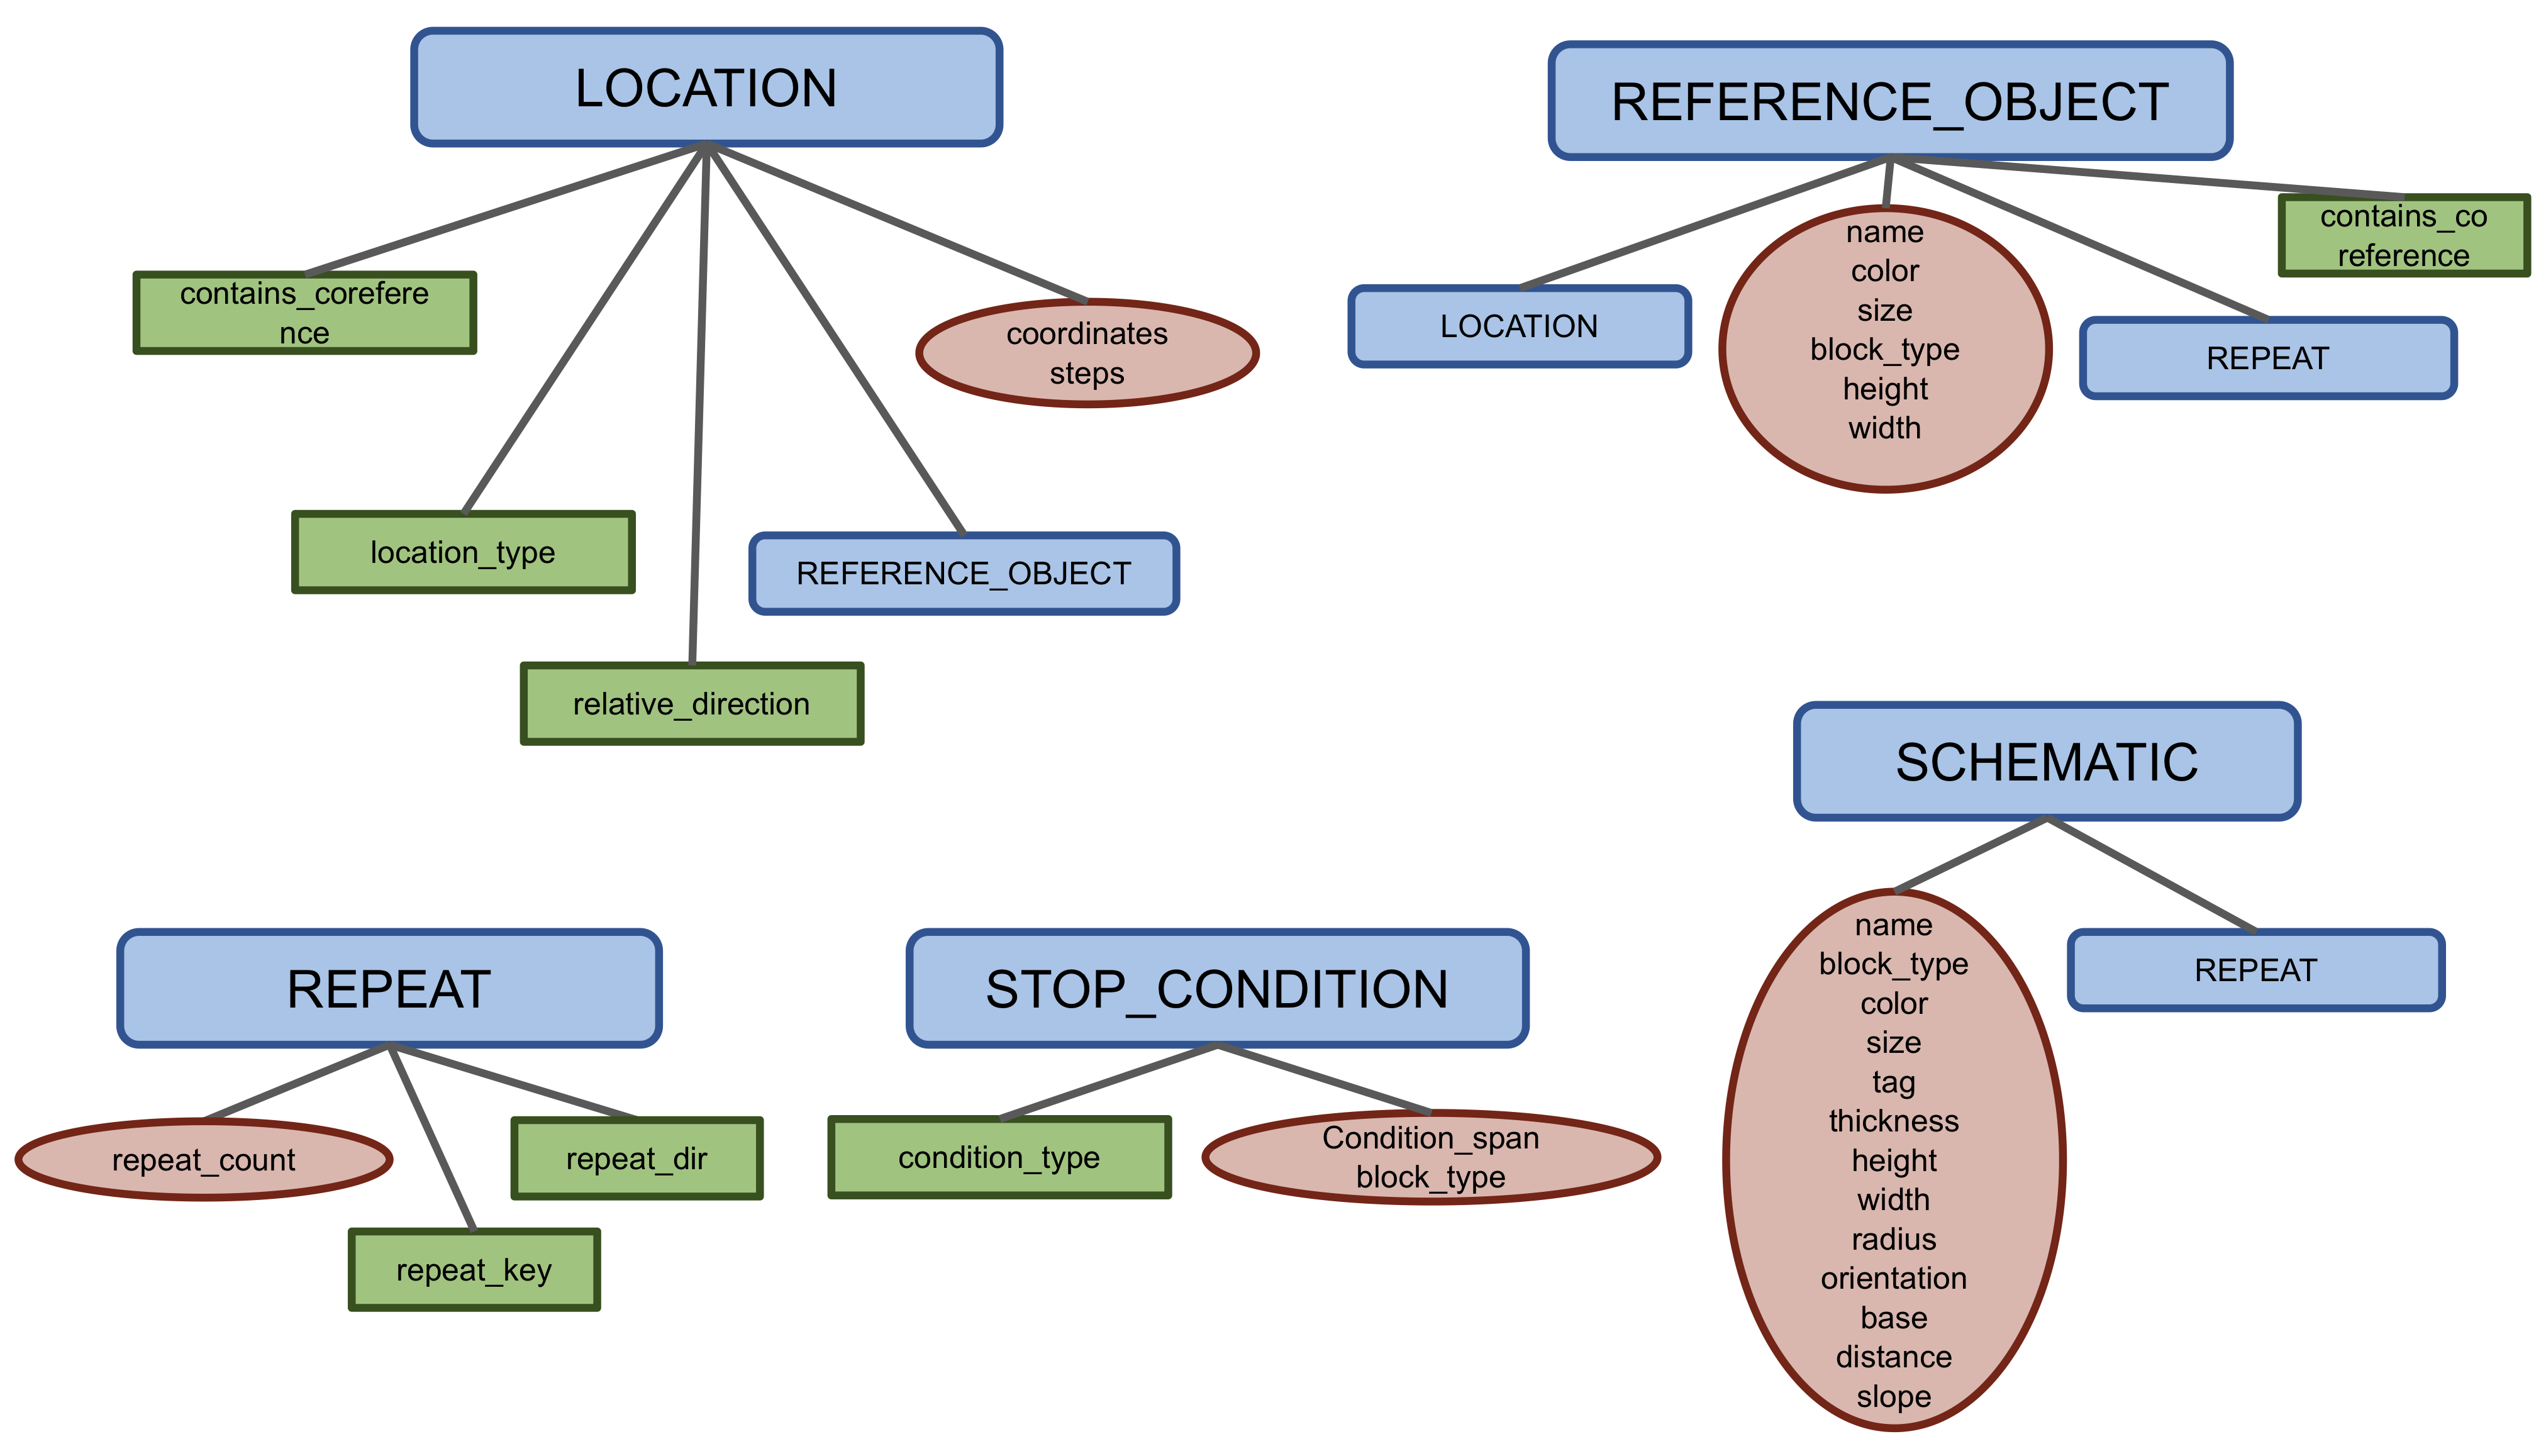
\includegraphics[width=\linewidth, height=6cm ]{figures/NOT_AS.png}
    \caption{The basic structure of internal nodes in the assistant's grammar.   Blue rectangles are internal nodes,  green rectangles are categorical leaf nodes, and red ovals are span nodes.      \label{fig:NOT_AS}}
\end{figure}

\smallskip

\noindent{\bf Memory interface: }  Finally, the assistant can interact with its SQL based memory.  It can place or update rows or cells, for example for tagging objects.  This can be considered a basic version of the self-improvement capabilities in \cite{kollar2013toward, thomason2015learning, wang2016learning, wang2017naturalizing}.    It can retrieve information for question answering similar to the VQA in \cite{yi2018neural}.

% We want to be able to add to this representation by allowing the user to \textsc{tag} existing objects with names or properties.  This can be considered a basic version of the self-improvement capabilities in \cite{kollar2013toward, thomason2015learning, wang2016learning, wang2017naturalizing}. Conversely, to query this internal state, we can ask the agent to \textsc{answer} questions about the world.  This part of the grammar is similar to the visual question-answering in \cite{yi2018neural}

\begin{figure*}
\center
 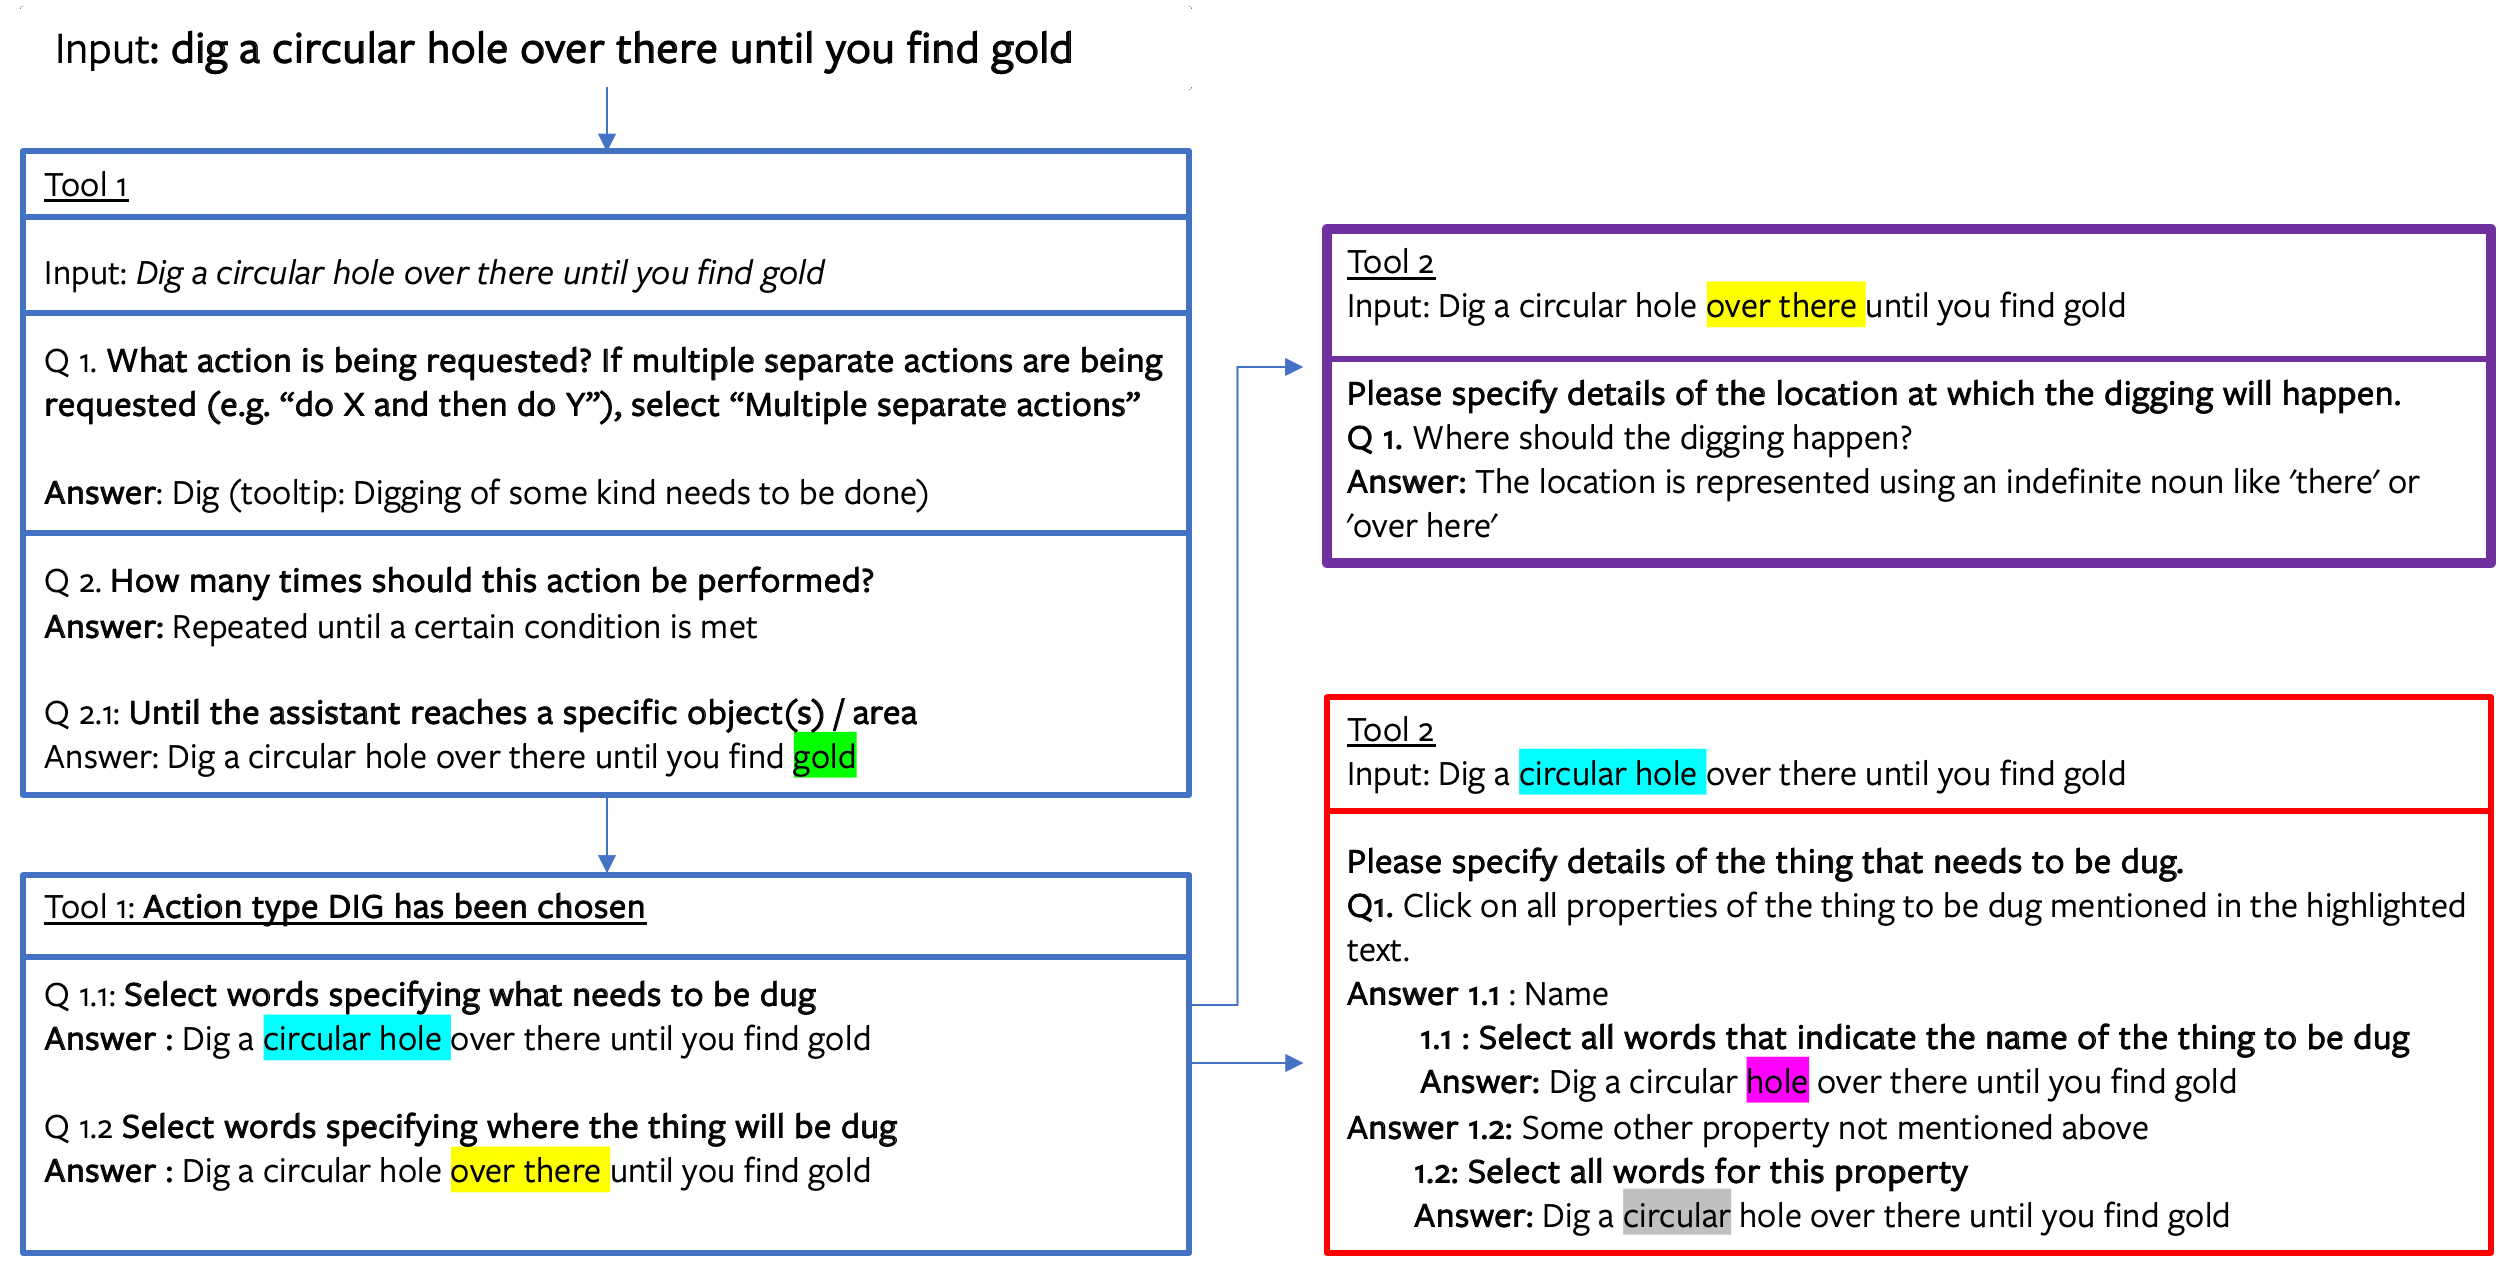
\includegraphics[width=\linewidth, height=6 cm  ]{figures/tools_diagram2.png}
 \caption{A representation of the annotation process using the web-based annotation tool described in Section \ref{sec:annotation}.  The colors of the boxes correspond to annotation tasks.  The highlighting on the text in the header of the later tasks is provided by a previous annotator.  We show more detailed screenshots of how the tool works in Appendix \ref{sec:anntn}}.
\label{fig:tool}
\end{figure*}

\subsection{Logical Forms}
The focus of this paper is an intermediate representation that allows natural language to be interpreted into programs over the basic actions from the previous section. 
The logical forms (represented as trees) making up this representation consist of three basic types of nodes: ``internal nodes'' that can have children, ``categorical'' (leaf) nodes that belong to a fixed set of possibilities, and ``span'' nodes that point to a region of text in the natural language utterance.   The full grammar is shown in the Appendix; and a partial schematic representation is shown in Figures \ref{fig:AS} and \ref{fig:NOT_AS}.  In the paragraphs below, we give more detail about some of the kinds of nodes in the grammar.     

We emphasize that this is an {\it intermediate} representation.   The logical forms do not come with any mechanism for generating language, and nodes do not correspond in any simple way with words.  On the other hand, the logical forms do not encode all of the information necessary for execution without the use of an interpreter that can access the assistant's memory and the Minecraft world state.   

%. Figure~\ref{fig:example_parse} presents an example parse tree for the \textsc{build} command \textit{``Make three oak wood houses to the left of the dark grey church.''}

\smallskip

\noindent{\bf Internal nodes: } Internal nodes are nodes that allow recursion; although most do not require it. 
 They can correspond to top-level actions, for example \textsc{Build}; in which case they would just be an ``action'' node with ``action\_type'' build; 
 see Figure \ref{fig:AS}.  They can also correspond to arguments to top-level actions, for example a ``reference\_object'', which specifies an object that has a spatial location.   
  Internal nodes are not generally required to have children;
   it is the job of the interpreter to deal with under-specified programs like a \textsc{Build} with no arguments. 

%Each action has a set of possible arguments, which themselves have a recursive argument structure. Each of these action types and complex arguments corresponds to an internal node (blue rounded rectangles in Figure~\ref{fig:example_parse}), with its children providing more specific information. For example, the \textsc{build} action can specify a \textsc{schematic} (what we want to build) and a \textsc{location} child (where we want to build it). In turn, the \textsc{schematic} can specify a general category (house, bridge, etc\ldots), as well as a set of properties (size, building material, etc...), and in our case also has a \textsc{repeat} child subtree specifying how many we want to build. Similarly, the \textsc{location} can specify an absolute location, a distance, direction, and information about the location \textsc{reference object} stored in a child subtree.

%One notable feature of this representation is that we do not know \textit{a priori} which of a node's possible children will be specified. For example, \textsc{build} can have a \textsc{schematic} and a \textsc{location} specified (\textit{``Build a house over there.''}), just a \textsc{schematic} (\textit{``Build a house.''}), just a \textsc{location} (\textit{``Build something next to the bridge.''}), or neither (\textit{``Make something.''}).

 In addition to the various \textsc{location}, \textsc{reference object}, \textsc{schematic}, and \textsc{repeat} nodes which can be found at various levels, another notable sub-tree is the action's \textsc{stop condition}, which essentially allows the agent to understand ``while'' loops (for example: ``dig down until you hit the bedrock'' or ``follow me'').  

\smallskip

\noindent{\bf Leaf nodes: } Eventually, arguments have to be specified in terms of values which correspond to (fixed) agent primitives. We call these nodes categorical leaves (green rectangles in Figures \ref{fig:AS} and \ref{fig:NOT_AS}).  As mentioned above, an ``action'' internal node has a categorical leaf child which specifies the \textbf{action type}. There are also \textbf{repeat type} nodes similarly specifying a kind of loop  for example in  the \textsc{repeat} sub-tree corresponding to "make three houses" the \textbf{repeat type} \textbf{for} specifies a ``for'' loop).   There are also \textbf{location type} nodes specifying if a location is determined by a reference object, a set of coordinates, etc.;  \textbf{relative direction} nodes that have values like ``left'' or ``right''. The complete list of categorical nodes is given in the Appendix.

However, there are limits to what we can represent with a pre-specified set of hard-coded primitives, especially if we want our agent to be able to learn new concepts or new values. Additionally, even when there is a pre-specified agent primitive, mapping some parts of the command to a specific value might be better left to an external module (e.g. mapping a number string to an integer value). For these reasons, we also have span leaves (red ovals in Figure~\ref{fig:NOT_AS}). %This way, a model can learn to generalize to e.g. colors or size descriptions that it has never seen before.   
For example, in the parse for the command  \textit{``Make three oak wood houses to the left of the dark grey church.''}, %starting from the ``action'' internal node, is {action: action_type: ``BUILD''
the \textsc{schematic} (an internal node) might be specified by the command sub-string corresponding to its \textbf{name} by the span``houses''  and the requested \textbf{block type} by the span ``oak wood''. The range of the for loop is specified by the \textsc{repeat}'s \textbf{for value} (``three''), and the \textsc{reference object} for the location is denoted in the command by its generic \textbf{name} and specific \textbf{color} with spans ``church'' and ``dark grey''.

 \smallskip

\noindent{\bf The root: } The root of the tree has three productions:   \textsc{put\_memory}, and \textsc{get\_memory}, corresponding to writing to memory and reading from memory; and \textsc{human\_give\_command} which also produces an \textsc{action\_sequence}, which is a special internal node whose children are ordered; multiple children correspond to an ordered  sequence of commands (``build a house and then a tower'').  In Figures \ref{fig:AS} and \ref{fig:NOT_AS} we show a schematic representation for an \textsc{action\_sequence}.